\section{Data and Analysis}
\label{sec:data}

In this section, we present the results of this study, considering
each of the two research questions. 

\subsection{RQ1 Analysis}

RQ1 investigates whether the use of the recommender system can 
improve the effectiveness of test case prioritization techniques.
%Figure~\ref{fig:All} shows the results combined for all applications.
Figure~\ref{fig:DASCP} presents the results for {\em DASCP}.
The vertical axis shows APFD scores, and the horizontal axis shows 
prioritization techniques:
``$T_{ch}$'' (change history-based), ``$T_{mfw}$'' (frequent web form-based), 
``$T_{mfm}$'' (frequent method-based), ``$T_{r}$'' (random order), 
``$T_{g}$'' (greedy technique), and 
``$T_{hcf}$'' (recommender system-based). 

\begin{figure}[!ht]
\vspace*{-10pt}
	\centering
	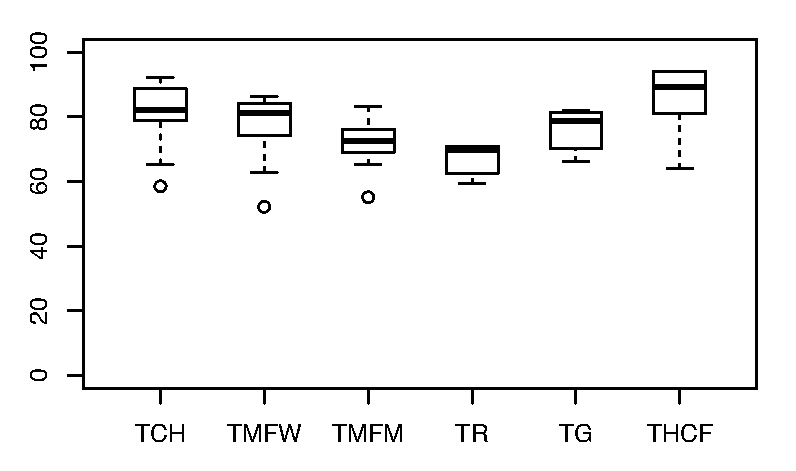
\includegraphics[width=0.90\linewidth]{./DASCPWGupdated.eps}
	\vspace*{-3pt}
	\caption{DASCP: APFD Boxplots}
	\label{fig:DASCP}
%\vspace*{-10pt}
\end{figure}

%Figure~\ref{fig:DASCP} presents the results for {\em DASCP}.
%Similar to the results that considered all applications, 
As can be seen the heuristic ($T_{hcf}$) outperformed all control techniques,
but data distribution patterns are different.  
%The variances are small, but there are more outliers.
Among control techniques, the random technique was 
the worst performer, whereas the frequent method-based technique ($T_{mfm}$)
produced results similar to the change history based technique ($T_{ch}$).


Figure~\ref{fig:nopCommerce} presents the results for {\em nopCommerce}.
The results show that our proposed technique outperformed  
all five control techniques, but the variance among the APFD scores is relatively high. 
Among the first three control techniques, the change history-based 
technique ($T_{ch}$) produced slightly better results than the others.
This application has 23 versions, and we had a sufficient
amount of change history data for our training, so we speculate that
this is the reason why the change history-based technique produced 
better results than the other control techniques. 
The greedy technique, which is the fifth control technique, did not yield 
better results than the other control techniques. 
The poor performance relative to other techniques could be explained by 
the nature of test cases of this application. A large number of test cases
have high code coverage, which caused the greedy technique which prioritizes based on 
block code coverage, to perform almost like the random technique.
 
\begin{figure}[!ht]
	\vspace*{-10pt}
	\centering
	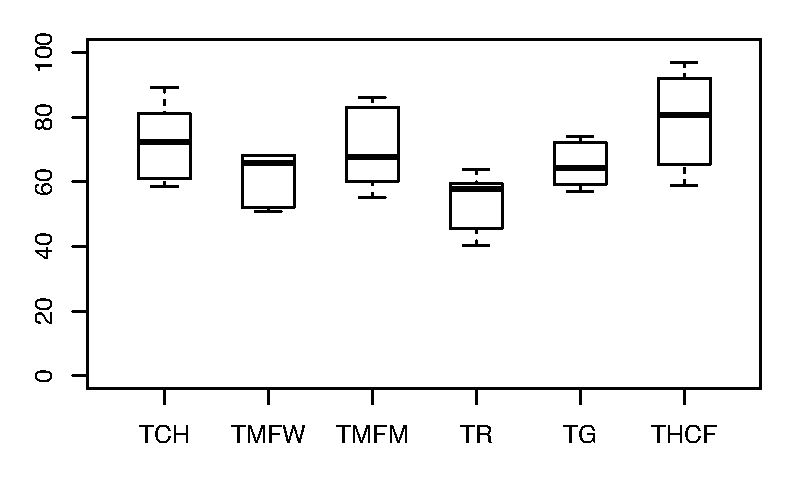
\includegraphics[width=0.90\linewidth]{./nopWG2updated.eps}
	\vspace*{-3pt}
	\caption{nopCommerce: APFD Boxplots}
	\label{fig:nopCommerce}
%\vspace*{-3pt}
\end{figure}

Figure~\ref{fig:Coevery} shows the results for {\em Coevery}. 
When we compared the median values, our heuristic technique improved
the rate of fault detection by 21\% over the four control techniques
($T_{ch}$, $T_{mfw}$ , $T_{mfm}$, and $T_{g}$) 
on average and 41\% over the random technique. 
Among the first three control techniques, $T_{ch}$ and $T_{mfw}$ 
produced slightly better results than $T_{mcf}$.

\begin{figure}[!ht]
	\vspace*{-10pt}
	\centering
	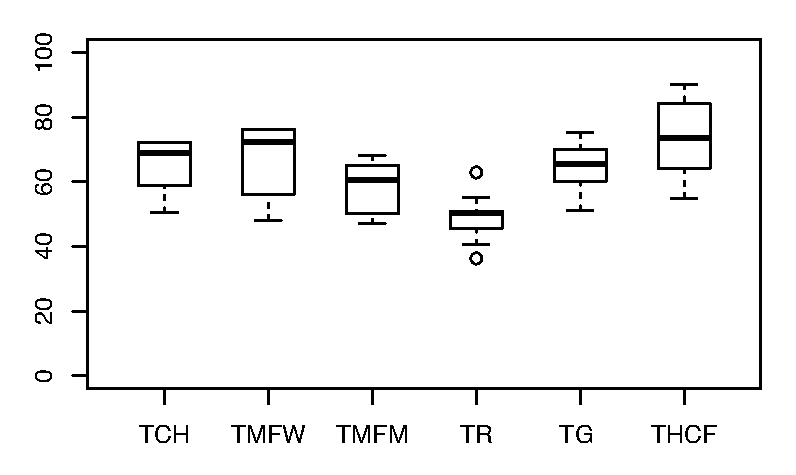
\includegraphics[width=0.90\linewidth]{./CoeveryWGupdated.eps}
	\vspace*{-3pt}
	\caption{Coevery: APFD Boxplots}
	\label{fig:Coevery}
%\vspace*{-10pt}
\end{figure}


Overall, the results showed that our proposed recommender 
system-based technique performed better than all the control techniques 
across all three applications. 
Among the control techniques, the random technique performed worst across all applications,
whereas the change history-based technique produced slightly better and more stable   
results for all applications.
Also, in the case of {\em DASCP} and {\em Coevery}, the greedy technique ($T_{g}$) 
showed marginally better results than other control techniques.

\begin{table*}[!ht]
\caption{NAPFD Scores on Average.}
\vspace*{-10pt}
\begin{center}
{\scriptsize
\begin{tabular}{|c|c|c|c|c|c|c||c|c|c|c|c|c|}\hline
Application & Test Exe. & \multicolumn{6}{c||} {Techniques} 
& \multicolumn{5}{c|} {Improvement Rate over Control} \\\hline \hline
& Rate (\%)  & $T_{ch}$ & $T_{mfw}$ & $T_{mfm}$ & $T_{r}$ & $T_{g}$ & $T_{hcf}$ 
& $T_{hcf}/T_{ch} $& $T_{hcf}/T_{mfw} $ & $T_{hcf}/T_{mfm}$ & $T_{hcf} /T_{r} $ &  $T_{hcf}/T_{g}$ \\\hline \hline
 
 
 &10	&18.54	&12.17	&15.12	&14.33	&16.53	&23.37	&26\%	&92\%	&54\%	&63\%	&41\%	\\
 &20	&21.31	&12.88	&16.78	&15.51	&25.13	&29.98	&40\%	&132\%	&78\%	&93\%	&19\%	\\
 &30	&28.86	&21.19	&25.12	&18.47	&36.42	&40.95	&41\%	&93\%	&63\%	&121\%	&12\%	\\
 &40	&40.42	&29.86	&38.68	&25.59	&41.02	&55.3	&36\%	&85\%	&42\%	&116\%	&34\%	\\
 DASCP &50	&54.34	&36.21	&42.9	&39.15	&50.13	&67.07	&23\%	&85\%	&56\%	&71\%	&33\%	\\
 &60	&61.7	&47.31	&50.34	&45.29	&54.38	&70.42	&14\%	&48\%	&39\%	&55\%	&29\%	\\
 &70	&68.34	&56.96	&65.97	&60.74	&62.36	&76.67	&12\%	&34\%	&16\%	&26\%	&22\%	\\
 &80	&75.41	&69.04	&71.14	&64.88	&72.4	&84.01	&11\%	&21\%	&18\%	&29\%	&16\%	\\
 &90	&83.35	&77.28	&77.69	&67.11	&78.4	&89.83	&7\%	&16\%	&15\%	&33\%	&14\%	\\
 &100	&90.16	&84.21	&79.22	&70.91	&82.12	&94.14	&4\%	&11\%	&18\%	&32\%	&14\%	\\\hline \hline
 
 &10	&17.54	&12.17	&15.75	&8.33	&12.25	&28.14	&60\%	&131\%	&78\%	&237\%	&129\%   \\
 &20	&29.28	&19.88	&28.35	&12.51	&22.39	&47.9	&63\%	&140\%	&68\%	&282\%	&113\%	\\
 &30	&38.86	&27.19	&35.45	&15.57	&40.12	&55.28	&42\%	&103\%	&55\%	&255\%	&37\%	\\
 &40	&44.42	&34.86	&48.68	&27.59	&48.66	&65.06	&46\%	&86\%	&33\%	&135\%	&33\%	\\
 nopCommerce &50	&58.34	&39.16	&54.94	&35.91	&53.26	&74.78	&28\%	&90\%	&36\%	&108\%	&40\%	\\
 &60	&62.7	&51.42	&57.08	&41.45	&60.62	&81.49	&29\%	&58\%	&42\%	&96\%	&34\%	\\
 &70	&68.14	&55.03	&59.97	&50.02	&69.23	&86.38	&26\%	&56\%   &44\%	&72\%	&24\%	\\
 &80	&76.22	&60.21	&64.14	&58.15	&71.5	&89.87	&17\%	&49\%	&40\%	&54\%	&25\%	\\
 &90	&79.4	&66.01	&70.22	&60.17	&73.66	&95.14	&19\%	&44\%	&35\%	&58\%	&29\%	\\
 &100	&82.16	&68.32	&76.04	&63.91	&74.13	&97.06	&18\%	&42\%	&27\%	&51\%	&30\%	\\\hline \hline
 
 &10	&26.54	&23.17	&29.12	&20.33	&24.45	&41.02	&54\%	&77\%	&40\%&	101\%	&67\%	\\
 &20	&44.28	&42.88	&45.12	&24.51	&42.12	&66.98	&51\%	&56\%	&48\%	&173\%	&59\%	\\
 &30	&60.86	&44.19	&50.12	&28.57	&58.18	&73.28	&20\%	&65\%	&46\%	&156\%	&25\%	\\
 &40	&63.42	&51.51	&53.68	&31.59	&63.4	&75.06	&18\%	&45\%	&39\%	&137\%	&18\%	\\
 Coevery &50	&64.34	&55.74	&58.3	&39.62	&64.73	&77.1	&19\%	&38\% 	&32\%	&94\%	&19\%	\\
 &60	&66.7	&56.33	&60.41	&44.09	&66.23	&78.65	&17\%	&39\% 	&30\%	&78\%	&18\%	\\
 &70	&68.19	&59.86	&62.97	&46.11	&69.07	&81.13	&18\%	&35\%	&28\%	&75\%	&17\%	\\
 &80	&70.67	&66.1	&65.14	&57.91	&73.19	&83.2	&17\%	&25\%	&27\%	&43\%	&13\%	\\
 &90	&71.81	&73.14	&66.03	&59.01	&74.36	&86.69	&20\%	&18\%	&31\%	&46\%	&16\%	\\
 &100	&72.16	&76.21	&68.22	&62.91	&75.15	&87.23	&20\%	&14\% 	&27\%	&38\%	&16\%	\\\hline  
 
% &10	&18.54	&12.17	&15.12	&14.33	&23.37 	&26\%	&92\%	&54\%	&63\%	\\
% &20	&21.31	&12.88	&16.78	&15.51	&29.98 	&40\%	&132\%	&78\%	&93\%	\\
% &30	&28.86	&21.19	&25.12	&18.47	&40.95 	&41\%	&93\%	&63\%	&121\%	\\
% &40	&40.42	&29.86	&38.68	&25.59	&55.3   &36\%	&85\%	&42\%	&116\%	\\
% DASCP &50	&54.34	&36.21	&42.9	&39.15	&67.07	&23\%	&85\%	&56\%	&71\%	\\
% &60	&61.7	&47.31	&50.34	&45.29	&70.42	&14\%	&48\%	&39\%	&55\%	\\
% &70	&68.34	&56.96	&65.97	&60.74	&76.67	&12\%	&34\%	&16\%	&26\%	\\
% &80	&75.41	&69.04	&71.14	&64.88	&84.01	&11\%	&21\%	&18\%	&29\%	\\
% &90	&83.35	&77.28	&77.69	&67.11	&89.83	&7\%	&16\%	&15\%	&33\%	\\
% &100	&90.16	&84.21	&79.22	&70.91	&94.14	&4\%	&11\%	&18\%	&32\%	\\\hline \hline
% 
%&10	&17.54	&12.17	&15.75	&8.33	&28.14	&60\%	&131\%	&78\%	&237\%	\\
%&20	&29.28	&19.88	&28.35	&12.51	&47.9	&63\%	&140\%	&68\%	&282\%	\\
%&30	&38.86	&27.19	&35.45	&15.57	&55.28	&42\%	&103\%	&55\%	&255\%	\\
%&40	&44.42	&34.86	&48.68	&27.59	&65.06	&46\%	&86\%	&33\%	&135\%	\\
%nopCommerce&50	&58.34	&39.16	&54.94	&35.91	&74.78	&28\%	&90\%	&36\%	&108\%	\\
%&60	&62.7	&51.42	&57.08	&41.45	&81.49	&29\%	&58\%   &42\%	&96\%	\\
%&70	&68.14	&55.03	&59.97	&50.02	&86.38	&26\%	&56\%   &44\%	&72\%	\\
%&80	&76.22	&60.21	&64.14	&58.15	&89.87	&17\%	&49\%	&40\%	&54\%	\\
%&90	&79.4	&66.01	&70.22	&60.17	&95.14	&19\%	&44\%	&35\%	&58\%	\\
%&100	&82.16	&68.32	&76.04	&63.91	&97.06	&18\%	&42\%	&27\%	&51\%	\\\hline \hline
%
%&10	&26.54	&23.17	&29.12	&20.33	&41.02	&54\%	&77\%	&40\%&	101\%	\\
%&20	&44.28	&42.88	&45.12	&24.51	&66.98	&51\%	&56\%	&48\%	&173\% \\
%&30	&60.86	&44.19	&50.12	&28.57	&73.28	&20\%	&65\%	&46\%	&156\%	\\
%&40	&63.42	&51.51	&53.68	&31.59	&75.06	&18\%	&45\%	&39\%	&137\%	\\
%Coevery &50	&64.34	&55.74	&58.3	&39.62	&77.1	&19\%	&38\% 	&32\%&	94\%	\\
%&60	&66.7	&56.33	&60.41	&44.09	&78.65	&17\%	&39\% 	&30\%	&78\%\\
%&70	&68.19	&59.86	&62.97	&46.11	&81.13	&18\%	&35\%	&28\%	&75\%	\\
%&80	&70.67	&66.1	&65.14	&57.91	&83.2	&17\%	&25\%	&27\%	&43\%	\\
%&90	&71.81	&73.14	&66.03	&59.01	&86.69	&20\%	&18\%	&31\%	&46\%	\\
%&100	&72.16	&76.21	&68.22	&62.91	&87.23	&20\%	&14\% 	&27\%	&38\%	\\\hline 

\end{tabular}
}
\end {center}
\label{tab:napfd}
\vspace*{-5pt}
\end{table*}

\subsection{RQ2 Analysis}

RQ2 investigates whether the use of the recommender system can improve the 
effectiveness of test prioritization when we have a limited budget for testing,
a common situation that the software industry often faces.

In RQ2 analysis, we measured the NAPFD, which is a normalized ratio of APFD, when 
our resources were not consistent.
In this experiment, first we executed 10\% of our test cases, and we continued to execute the
test cases in increments of 10\% of the total until they had all been  
executed to see whether we could improve the fault detection rate, given a 
time constraint dictating that running 100\% of the test cases at one time was not feasible. 

Table~\ref{tab:napfd} shows the results of our three applications.
This table shows the results of two primary analyses. The first part of the table 
presents the NAPFD scores on average, and the second part shows the 
improvement rates of the heuristic technique over the five other control techniques. 

By examining the numbers in the table, we can observe that the improvement
rates of our heuristic technique over the control techniques vary widely. 
When we compared the heuristic with $T_{ch}$, the improvement rates ranged from
4\% to 41\% for {\em DASCP}, from 17\% to 63\% for {\em nopCommerce}, and from 17\% to 54\%
for {\em Coevery}.
When compared with $T_{mfw}$, the improvement rates ranged from
11\% to 132\% for {\em DASCP}, from 42\% to 140\% for {\em nopCommerce}, and from 14\% to 77\%
for {\em Coevery}, indicating significant improvements. 
When compared with $T_{mfm}$, the improvement rates ranged from
15\% to 78\% for {\em DASCP}, from 27\% to 78\% for {\em nopCommerce}, and from 27\% to 48\%
for {\em Coevery}, indicating results similar to those for as $T_{ch}$.
When compared with $T_{g}$, the improvement rates ranged from
12\% to 41\% for {\em DASCP}, from 24\% to 129\% for {\em nopCommerce}, and from 13\% to 67\%
for {\em Coevery}, showing improvement over a popular and commonly used technique.
As for the comparison with $T_{r}$, the results were more remarkable.
The rates ranged from 32\% to 282\% for all three applications. 

One outstanding trend we observed in the table is that the improvement 
rates are much higher when the time budget is smaller.
For example, in the comparison with $T_{ch}$ for {\em nopCommerce}, 
when 10\% of the budget was assigned, the improvement rate was 60\%,
but when we had a full budget, the rate dropped to 18\%.
A similar trend can be observed across all control techniques and applications.  
This indicates that our approach can be more helpful when companies are operating
under a tight budget.

